\documentclass{standalone}
\usepackage{tikz}
\usetikzlibrary{patterns}

\begin{document}

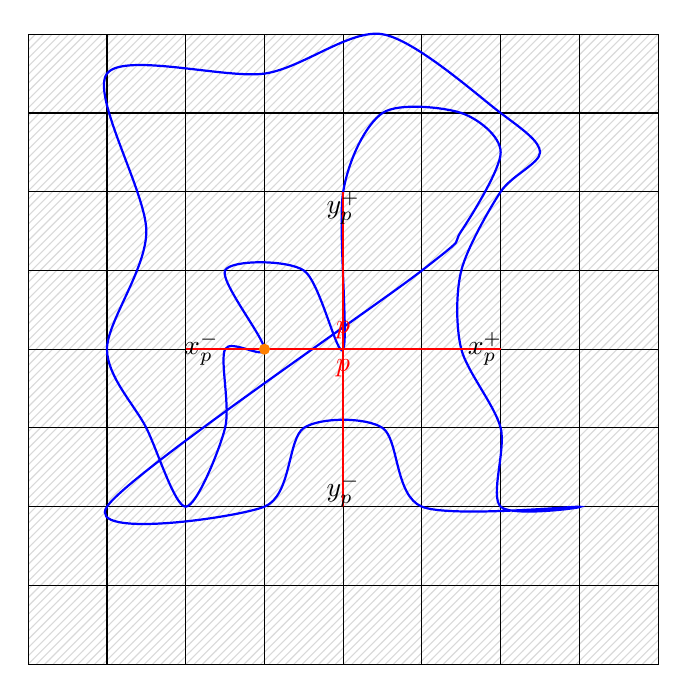
\begin{tikzpicture}
    % Grid pattern
    \draw[pattern=north east lines, pattern color=gray!30] (-4,-4) rectangle (4,4);
    \foreach \x in {-3,...,3} {
        \draw (\x,-4) -- (\x,4);
        \draw (-4,\x) -- (4,\x);
    }

    % Poorly textured region outline
    \draw[blue, thick] plot [smooth cycle] coordinates {(-3,-2) (-1,-2) (-0.5,-1) (0.5,-1) (1,-2) (3,-2) (2,-2) (2,-1) (1.5,0) (1.5,1) (2,2) (2.5,2.5) (2,3) (0.5,4) (-1,3.5) (-3,3.5) (-2.5,1.5) (-3,0) (-2.5,-1) (-2,-2) (-1.5,-1) (-1.5,0) (-1,0) (-1.5,1) (-0.5,1) (0,0) (0,2) (0.5,3) (1.5,3) (2,2.5) (1.5,1.5) (1,1) };

    % Red lines and annotations
    \draw[red, thick] (-2,0) -- (2,0) node [midway, below] {$p$};
    \draw[red, thick] (0,-2) -- (0,2) node [midway, above] {$p$};

    % Annotations for x and y
    \node at (-1.8,0) {$x_{p}^{-}$};
    \node at (1.8,0) {$x_{p}^{+}$};
    \node at (0,-1.8) {$y_{p}^{-}$};
    \node at (0,1.8) {$y_{p}^{+}$};

    % Orange point indicating problematic pixels
    \fill[orange] (-1,0) circle (2pt);

\end{tikzpicture}

\end{document}